\documentclass[aspectratio=169,11pt]{beamer}
\usepackage[T1]{fontenc}
\usepackage[utf8]{inputenc}
\usepackage[french]{babel}
\usepackage{lmodern}
\usepackage{graphicx}
\usepackage{booktabs}
\usepackage{tabularx}
\definecolor{navy}{HTML}{103B50}
\definecolor{teal}{HTML}{087F8C}
\setbeamercolor{structure}{fg=teal}
\setbeamercolor{frametitle}{fg=navy}
\setbeamercolor{normal text}{fg=navy,bg=white}
\setbeamertemplate{navigation symbols}{}
\setbeamertemplate{footline}{\hfill\insertframenumber\,/\,\inserttotalframenumber\hspace{6mm}\vspace{3mm}}
\setbeamerfont{frametitle}{size=\Large,series=\bfseries}
\setbeamersize{text margin left=8mm,text margin right=8mm}
\setbeamertemplate{itemize items}[circle]
\graphicspath{{images/}}
\begin{document}
\begin{frame}[plain]
\relax
{\LARGE\bfseries Contrôle décentralisé d’un essaim de robots\par}\vspace{5mm}
Réseaux de neurones sur graphe\par\vspace{2mm}
Mémoire de Master · Informatique\par\vspace{2mm}
Intelligence artificielle et Sciences des données\par\vspace{2mm}
MWANAMPUTU LABEYA Laurent\par\vspace{2mm}
Université de Kinshasa · 2025–2026\par\vspace{2mm}
Directeur · Prof. Dr Selain KASEREKA KABUNGA\par\vspace{2mm}
\note{Présenter le sujet. Il s’agit d’une étude en simulation 2D, avec apprentissage supervisé par imitation. Annoncer une présentation de 15 à 20 minutes, hors questions. Source : page de garde et introduction du mémoire.}
\end{frame}

\begin{frame}{Coordonner des décisions locales}
\begin{itemize}\setlength{\itemsep}{4mm}
\item Chaque robot observe son état et ses voisins à portée
\item Le groupe doit former une figure et éviter les contacts
\item La difficulté augmente avec l’effectif et les obstacles
\item Question étudiée : un GAT peut-il apprendre une commande locale utile ?
\end{itemize}
\note{Distinguer la commande locale du calcul de la mission partagée. La navigation utilise une carte connue et un planificateur classique. Ne pas présenter toute la chaîne comme apprise. Source : introduction et méthodologie.}
\end{frame}

\begin{frame}{Objectifs et démarche}
\begin{itemize}\setlength{\itemsep}{4mm}
\item Construire un simulateur physique 2D
\item Attribuer les places par échanges locaux
\item Apprendre les accélérations à partir d’exemples
\item Comparer aux règles classiques sur des essais réservés
\end{itemize}
\note{Le résultat attendu est une évaluation mesurée, avec ses limites. Les tests du code et les essais du modèle répondent à deux questions différentes. Source : introduction, objectifs et méthodes.}
\end{frame}

\begin{frame}{Un simulateur dans un plan 2D}
\begin{columns}[T]\begin{column}{0.45\textwidth}
\begin{itemize}\setlength{\itemsep}{4mm}
\item Position (x, y), vitesse et accélération
\item Robots représentés par des disques de rayon 0,10 m
\item Pas de temps 0,10 s · portée de communication 3 m
\item Vitesse $\leq$ 1 m/s · accélération $\leq$ 2 m/s$^2$
\end{itemize}
\end{column}\begin{column}{0.53\textwidth}\centering
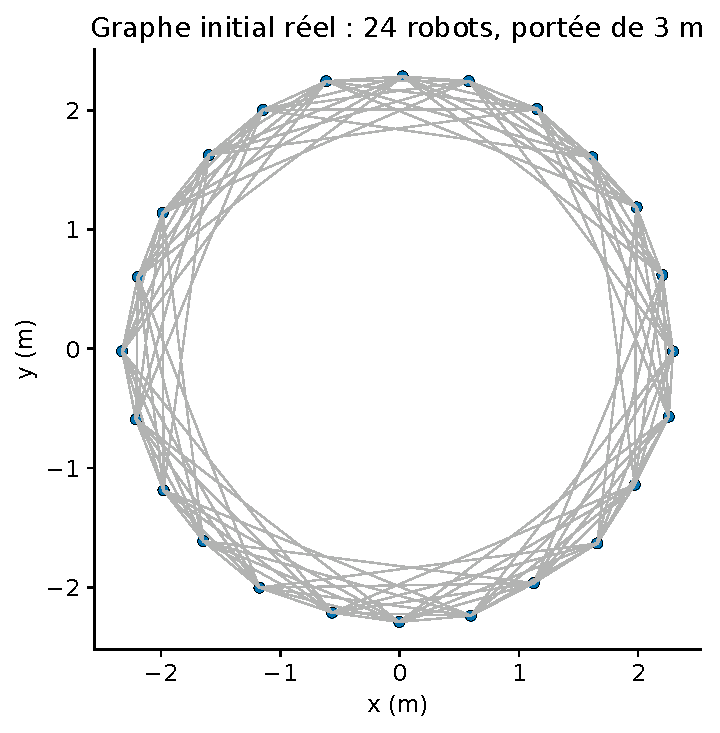
\includegraphics[width=\linewidth,height=5.4cm,keepaspectratio]{current_graph.pdf}
\end{column}\end{columns}
\note{Aucun mouvement vertical ni modèle physique 3D. Les observations viennent des états simulés, sans caméra ni LiDAR réel. Figure du graphe calculée à partir du programme. Source : méthodologie, paramètres physiques ; latex/images/current\_graph.png.}
\end{frame}

\begin{frame}{Préparer, attribuer, puis construire}
\begin{itemize}\setlength{\itemsep}{4mm}
\item 1  Rejoindre le cercle de rendez-vous
\item 2  Freiner et échanger les demandes de places
\item 3  Résoudre les conflits de réservation
\item 4  Rejoindre la figure choisie
\item 5  Transporter la formation si la mission le demande
\end{itemize}
\note{Le cercle est programmé. Il n’est pas une décision spontanée du réseau. L’attribution classe les places par distance ; les identifiants départagent les conflits. Les numéros ne sont pas des entrées du réseau. Source : protocole, guide des expériences.}
\end{frame}

\begin{frame}{Le réseau propose une accélération}
\begin{itemize}\setlength{\itemsep}{4mm}
\item État propre et cible locale $\rightarrow$ encodage
\item États relatifs des voisins $\rightarrow$ attention et agrégation
\item Le même réseau est utilisé par tous les robots
\item GAT protégé : un filtre classique vérifie la commande
\item GAT structuré : base attractive et corrections apprises
\end{itemize}
\note{Un GAT est un Graph Attention Network. L’attention pondère les informations des voisins. Le modèle ne choisit pas les places à la place du protocole. Le planificateur de navigation est également classique. Source : méthodologie, architecture et commande finale.}
\end{frame}

\begin{frame}{Des données synthétiques pour l’imitation}
\begin{itemize}\setlength{\itemsep}{4mm}
\item Le simulateur produit des situations et leurs observations
\item Le contrôleur de référence fournit l’accélération attendue
\item 531 360 observations locales pour l’entraînement initial
\item 53 136 observations pour la validation
\item Séparation des fichiers et des départs à examiner
\end{itemize}
\note{Ces nombres concernent le GAT initial. Les fichiers d’entraînement sont 185, validation 20, test 9. Beaucoup d’observations d’une même trajectoire ne représentent pas autant d’essais indépendants. Le test initial réutilise un départ sur neuf formes. Source : run.json initial et méthodologie.}
\end{frame}

\begin{frame}{Entraîner ne garantit pas la mission}
\begin{itemize}\setlength{\itemsep}{4mm}
\item Apprentissage supervisé par régression
\item MSE entre accélération prédite et accélération attendue
\item La validation sert à choisir le modèle conservé
\item Le test réservé évalue le comportement complet
\item Une MSE faible ne garantit pas zéro contact
\end{itemize}
\note{MSE signifie erreur quadratique moyenne. Pas de matrice de confusion pour cette sortie continue. Le GAT initial est retenu à l’époque 11, après arrêt à l’époque 23. Ne pas comparer directement l’échelle de la MSE à celle de la perte composite structurée. Source : journaux d’entraînement et Figure 3.2.}
\end{frame}

\begin{frame}{Des critères pour une mission complète}
\vspace{3mm}\begin{tabularx}{\textwidth}{lX}\toprule
\textbf{Mesure} & \textbf{Condition ou usage}\\[2mm]
\midrule
Erreur de formation & Au plus 0,10 m pour stabiliser\\[2mm]
Vitesse résiduelle & Au plus 0,05 m/s pendant 1 s\\[2mm]
Contacts & Aucun sur l’essai complet\\[2mm]
Navigation & Destination $\leq$ 0,10 m ; déformation $\leq$ 0,20 m\\[2mm]
MSE & Erreur d’imitation pendant l’apprentissage\\[2mm]
\bottomrule\end{tabularx}
\note{Formation : erreur de couverture bidirectionnelle entre robots et places, pas seulement une distance moyenne. Les contacts sont vérifiés sur les déplacements entre états enregistrés. Les durées sont simulées. Source : section 3.11 du mémoire.}
\end{frame}

\begin{frame}{Le filtre change le bilan du GAT initial}
\begin{itemize}\setlength{\itemsep}{4mm}
\item Neuf cas réservés à douze robots
\item Un même départ réutilisé pour neuf formes
\end{itemize}
\vspace{3mm}\begin{tabularx}{\textwidth}{lXX}\toprule
\textbf{Commande} & \textbf{Réussites} & \textbf{Contacts}\\[2mm]
\midrule
Contrôleur de référence & 9/9 & 0\\[2mm]
GAT initial brut & 0/9 & 54\\[2mm]
GAT initial protégé & 9/9 & 0\\[2mm]
\bottomrule\end{tabularx}
\note{Résultats du rapport 008d-local-target-expanded-test.json. Le taux porte sur neuf cas, pas sur toutes les formes ni tous les départs. La préparation est classique. Le modèle protégé ne prouve pas la réussite du réseau seul.}
\end{frame}

\begin{frame}{Une figure précise peut avoir subi des contacts}
\begin{columns}[T]\begin{column}{0.45\textwidth}
\begin{itemize}\setlength{\itemsep}{4mm}
\item Ellipse · 12 robots · départ 7300
\item GAT brut et protégé finissent à environ 9,28 mm d’erreur
\item Brut : 5 contacts · protégé : aucun
\item Ce cas appartient déjà aux neuf essais précédents
\end{itemize}
\end{column}\begin{column}{0.53\textwidth}\centering
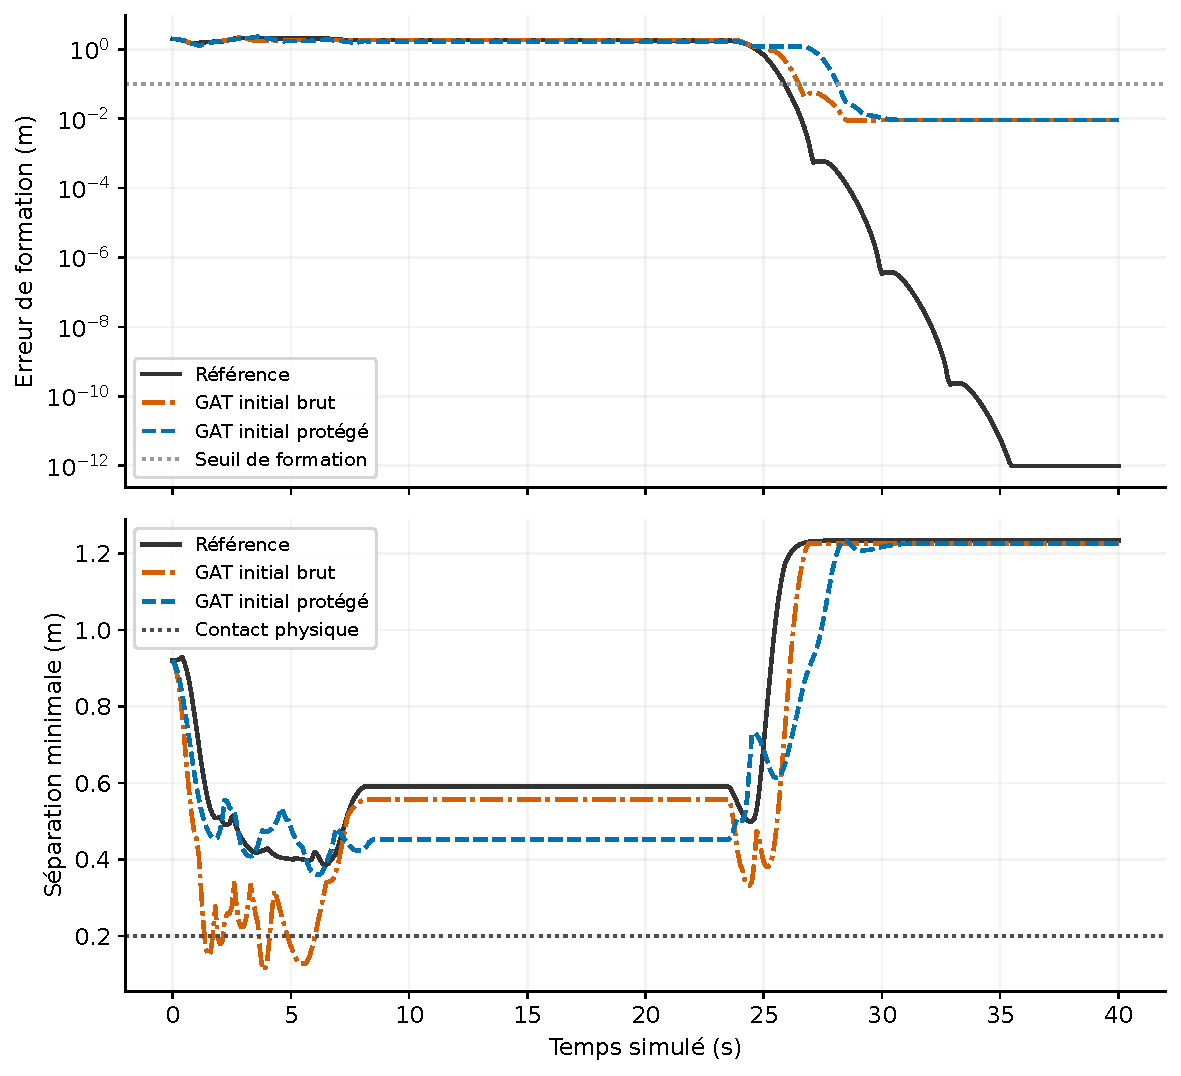
\includegraphics[width=\linewidth,height=5.4cm,keepaspectratio]{current_ellipse_case.pdf}
\end{column}\end{columns}
\note{Source : rapport 008d, cas geometries\_ellipse graine 7300 et archives NPZ associées. Le graphe montre l’erreur et la séparation minimale. Le seuil de contact est 0,20 m entre centres. Le tracé logarithmique borne les très petites erreurs à 10⁻¹$^2$ m pour l’affichage seulement.}
\end{frame}

\begin{frame}{Le modèle structuré réussit les 18 cas réservés}
\begin{itemize}\setlength{\itemsep}{4mm}
\item Rectangle, lettre C et nombre 3
\item Deux départs par effectif · six configurations initiales distinctes
\item Sans filtre pendant les phases de mouvement apprises
\end{itemize}
\vspace{3mm}\begin{tabularx}{\textwidth}{lXX}\toprule
\textbf{Effectif} & \textbf{Réussites} & \textbf{Contacts}\\[2mm]
\midrule
12 robots & 6/6 & 0\\[2mm]
24 robots & 6/6 & 0\\[2mm]
64 robots & 6/6 & 0\\[2mm]
\bottomrule\end{tabularx}
\note{Source : 014-vector-fresh-test.json et audit final. Six cas par effectif : trois formes fois deux graines. Les départs sont proches d’un rendez-vous contrôlé ; il ne s’agit pas de départs arbitraires. La préparation et l’attribution restent classiques.}
\end{frame}

\begin{frame}{À 64 robots, l’attribution coûte du temps}
\begin{columns}[T]\begin{column}{0.45\textwidth}
\begin{itemize}\setlength{\itemsep}{4mm}
\item Jusqu’à N$^2$ tours locaux de 0,10 s
\item Attribution à 64 robots : 409,6 s simulées
\item Stabilisation moyenne complète : 465,8 s
\item Le protocole d’attribution est une piste d’amélioration
\end{itemize}
\end{column}\begin{column}{0.53\textwidth}\centering
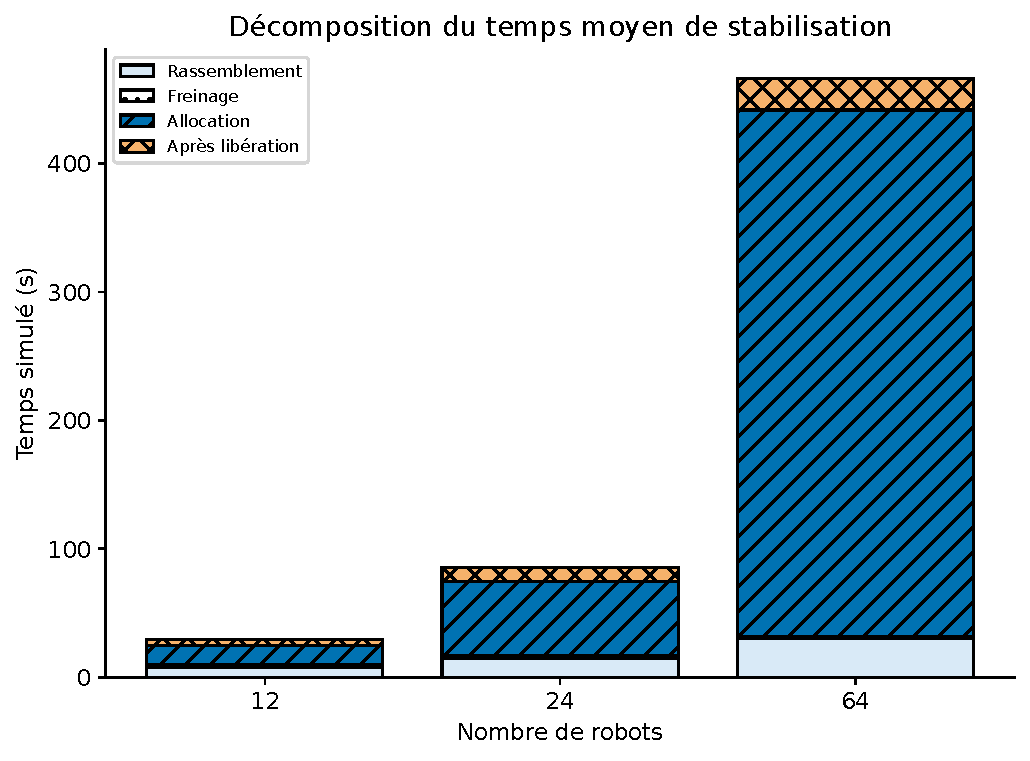
\includegraphics[width=\linewidth,height=5.4cm,keepaspectratio]{current_timing.pdf}
\end{column}\end{columns}
\note{Source : résultats structurés 014, Figure de décomposition des durées. À 12 robots, stabilisation moyenne 29,43 s ; à 24, 85,23 s. Ne pas confondre temps simulé et temps d’attente réel devant l’ordinateur.}
\end{frame}

\begin{frame}{Navigation près de cinq à dix obstacles}
\begin{columns}[T]\begin{column}{0.45\textwidth}
\begin{itemize}\setlength{\itemsep}{4mm}
\item Carré de douze robots · carte connue
\item Détour calculé pour toute la largeur du groupe
\item Huit cas par contrôleur, tous réussis sans contact
\item Comparaison classique / GAT initial protégé
\end{itemize}
\end{column}\begin{column}{0.53\textwidth}\centering
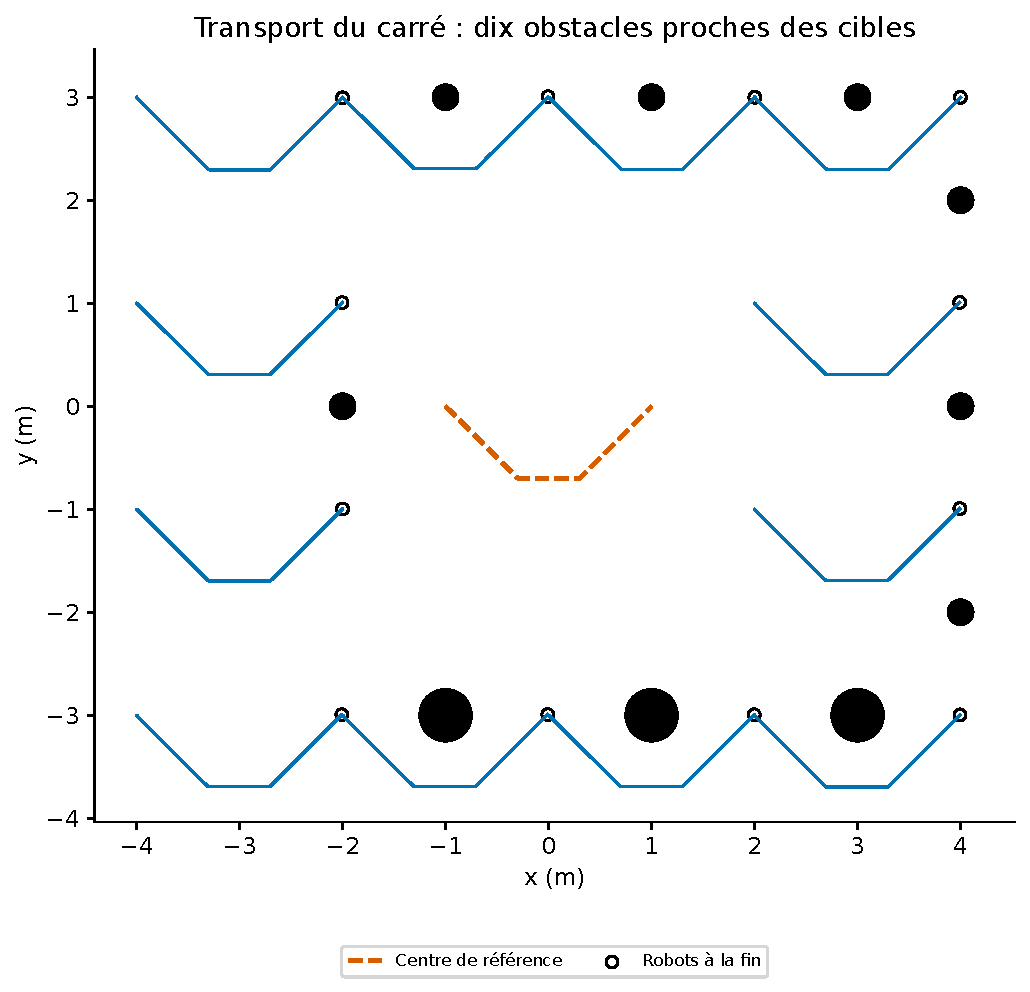
\includegraphics[width=\linewidth,height=5.4cm,keepaspectratio]{current_navigation.pdf}
\end{column}\end{columns}
\note{Source : 019-near-targets-evaluation.json et audit. Les huit cas comprennent les nombres 5 à 10, un second départ à 10 et une régression à un obstacle. Le visuel illustre le cas à dix obstacles. Le GAT structuré brut n’est pas évalué en navigation.}
\end{frame}

\begin{frame}{Un catalogue plus large que les essais réservés}
\begin{columns}[T]\begin{column}{0.45\textwidth}
\begin{itemize}\setlength{\itemsep}{4mm}
\item 26 lettres A–Z et dix nombres 1–10
\item Vingt noms de figures géométriques
\item 56 noms pour 54 géométries distinctes
\item Le catalogue disponible dépasse le domaine validé
\end{itemize}
\end{column}\begin{column}{0.53\textwidth}\centering
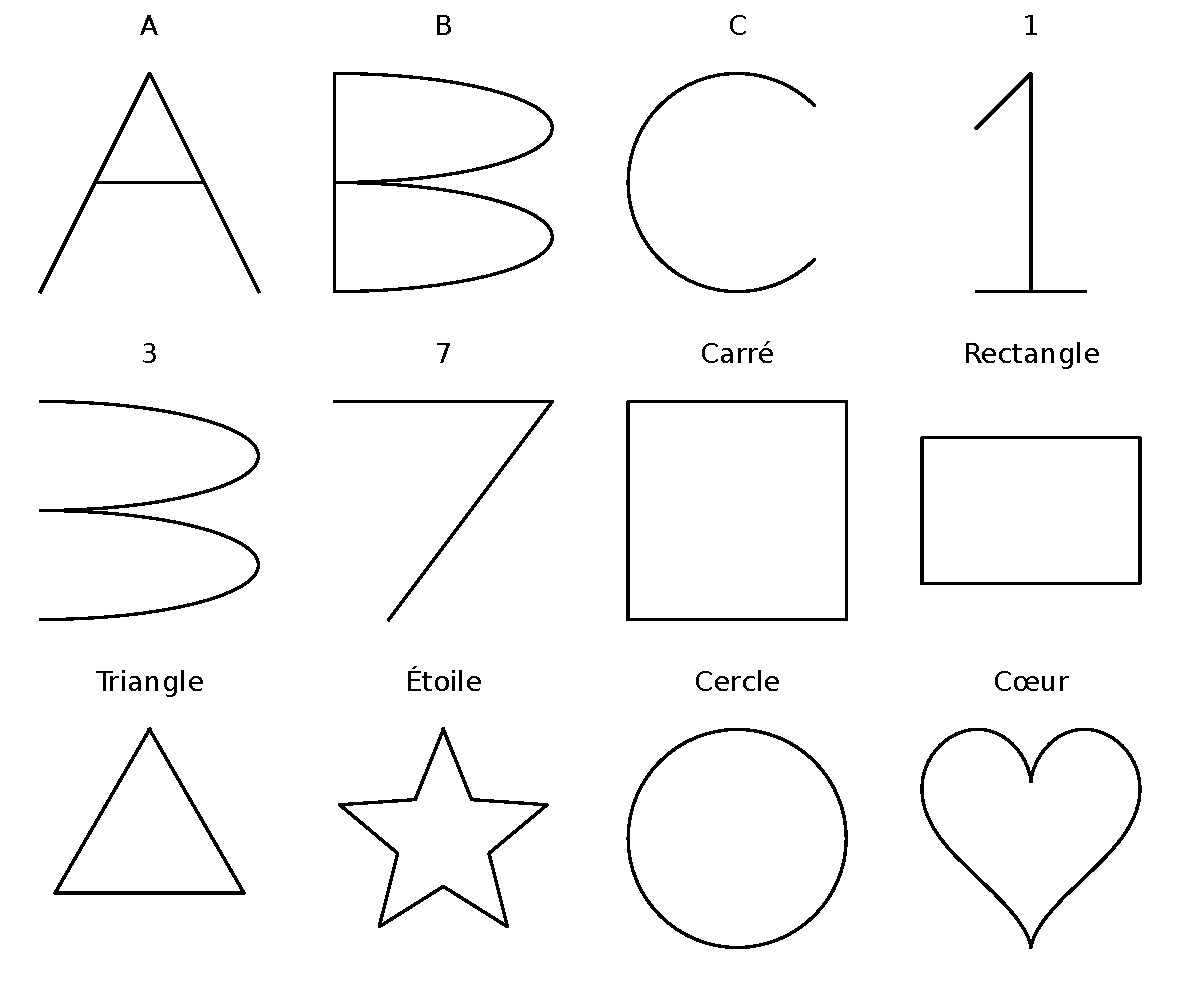
\includegraphics[width=\linewidth,height=5.4cm,keepaspectratio]{current_catalog.pdf}
\end{column}\end{columns}
\note{Source : catalogue du programme et Figure du mémoire. O et cercle partagent une géométrie ; V et la figure en V également. La génération d’une cible ne prouve pas la réussite du modèle sur cette cible.}
\end{frame}

\begin{frame}{Les limites de l’étude}
\begin{itemize}\setlength{\itemsep}{4mm}
\item Simulation 2D idéale, sans validation sur robots réels
\item Peu de configurations initiales indépendantes
\item Départs contrôlés pour le modèle structuré
\item Navigation aidée par une carte et un planificateur classiques
\item Pannes, bruit et pertes de messages non validés
\end{itemize}
\note{Présenter ces limites clairement. Le graphe local n’annule pas les hypothèses de préparation et de mission partagée. Les résultats obtenus valent pour les conditions enregistrées. Source : discussion, validité interne, externe et de construit.}
\end{frame}

\begin{frame}{Contributions et suite du travail}
\begin{itemize}\setlength{\itemsep}{4mm}
\item Une chaîne reproductible de simulation et d’évaluation
\item Des commandes apprises comparées à une référence classique
\item Des métriques qui conservent les échecs et les contacts
\item À poursuivre : départs variés, attribution plus rapide, bruit
\item Puis une validation progressive sur robots réels
\end{itemize}
\note{Conclure sur ce que les essais établissent réellement. Le réseau structuré est prometteur dans son domaine contrôlé. Les perspectives ne sont pas des résultats déjà obtenus. Source : conclusion générale.}
\end{frame}

\begin{frame}{Démonstration et échanges}
\begin{itemize}\setlength{\itemsep}{4mm}
\item Former un rectangle avec le modèle structuré
\item Comparer les commandes sur le même départ
\item Observer l’erreur, la stabilisation et les contacts
\item Montrer le détour près des obstacles
\item Merci pour votre attention
\end{itemize}
\note{Avant la soutenance, lancer le serveur puis ouvrir http://127.0.0.1:8765/. Préparer un résultat enregistré en cas d’indisponibilité de l’application. La démonstration illustre les résultats ; elle ne remplace pas la campagne d’évaluation. Slides 19 et 20 sont des compléments pour les questions.}
\end{frame}

\begin{frame}{Complément — Réserver une place}
\begin{itemize}\setlength{\itemsep}{4mm}
\item Chaque robot classe les places selon leur distance
\item Les demandes circulent entre voisins
\item En cas de conflit, l’identifiant prioritaire garde la place
\item L’autre robot demande sa place suivante
\item L’affectation et l’évitement physique ont des rôles distincts
\end{itemize}
\note{Exemple oral : les robots 2 et 5 demandent la même place. Le 2 conserve la demande prioritaire ; le 5 choisit la suivante. Un robot qui traverse une place ne devient pas automatiquement son propriétaire. Le réseau apprend la commande, pas cette réservation. Source : protocole d’attribution et guide.}
\end{frame}

\begin{frame}{Complément — Régression et classification}
\begin{itemize}\setlength{\itemsep}{4mm}
\item Classification : prédire une catégorie
\item Régression : prédire une valeur continue
\item Ici, la sortie est une accélération à deux composantes
\item La MSE mesure l’erreur d’imitation
\item Les essais de simulation mesurent la réussite physique
\end{itemize}
\note{Le rappel et la matrice de confusion conviennent à une tâche de classification avec catégories annotées. Ils ne sont pas nécessaires pour évaluer directement les accélérations continues de ce modèle. Succès/échec est un verdict de simulation, pas la sortie apprise. Source : concepts et critères d’évaluation.}
\end{frame}

\end{document}
